\documentclass{article}
\usepackage{amsmath}
\usepackage{amssymb}
\usepackage{graphicx}
\usepackage{hyperref}
\usepackage[version=4]{mhchem}

\title{Example 9}
\date{}

\begin{document}
\maketitle

In \(\triangle A B C, \angle A C B=90^{\circ} D\) is the midpoint of \(B C\). \(E\) is the midpoint of \(A D\). Extend \(C E\) to meet \(A B\) at \(F . F G / / A C\) and meet \(A D\) at \(G\).. Prove: \(F B=2 C G\).

Solution:
Take \(H\), the midpoint of \(B F\).\\
\centering
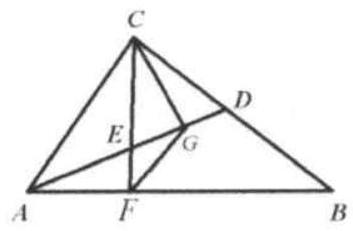
\includegraphics[width=\textwidth]{images/040(1).jpg}

Connect DH.\\
Since point \(D\) is the midpoint of \(B C\), by Theorem 2.1, \(D H / / C F / / E F\). Since \(E\) is the midpoint of \(A D\), by\\
Theorem 2.2. \(F\) is the midpoint of \(A H\).\\
So \(A F=F H=H B\).\\
Note that \(C E\) is the median of right triangle \(A C D\). So \(C E\)\\
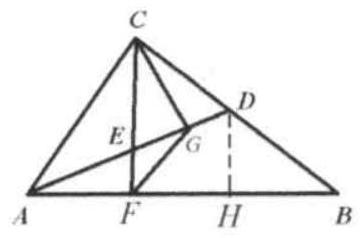
\includegraphics[width=\textwidth]{images/040.jpg} \(=A E\).\\
Therefore, \(\triangle A E C\) is an isosceles triangle with\\
\(\angle A C E=\angle C A E=\alpha\).\\
Since \(F G / / A C, \angle G F E=\angle A C E=\alpha\).\\
\(\angle F G E=\angle C A E=\alpha\).\\
Therefore, \(\triangle F G E\) is an isosceles triangle with \(E G=E F\).\\
\centering
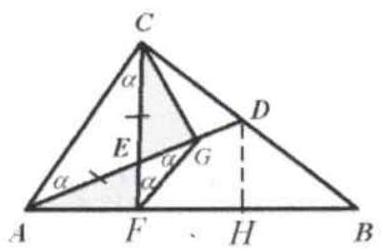
\includegraphics[width=\textwidth]{images/040(3).jpg}

We also know that \(\angle A E F=\angle C E G\).\\
Thus \(\triangle A E F \cong \triangle C E G\). \(C G=A F=F H=H B\), or \(F B=2 C G\).\\

\end{document}
